\section{Конструкторская часть}

\subsection{Определение требований к межсетевому экрану}
В соответствии с параграфом \ref{sec:task} межсетевой экран должен предоставлять следующие возможности:
\begin{itemize}
	\item добавление нового правила;

	\item удаление правила;
	
	\item просмотр всех правил;
	
	\item сокрытие модуля в системе;
	
	\item обнаружение модуля в системе. \\
\end{itemize}

Для непосредственного взаимодействия с пользователем необходимо разработать отдельную программу, представляющую из себя интерфейс для работы с загружаемым модулем. Программа выполняет не только функцию связующего звена между пользователем и межсетевым экраном, но и проверку входных данных: корректность вводимых команд и правил. \\

\subsection{Инициализация межсетевого экрана}
На Рисунке \ref{fig3:image} представлена подробная схема алгоритма инициализации межсетевого экрана.
\begin{figure}[p]
	\begin{center}
		{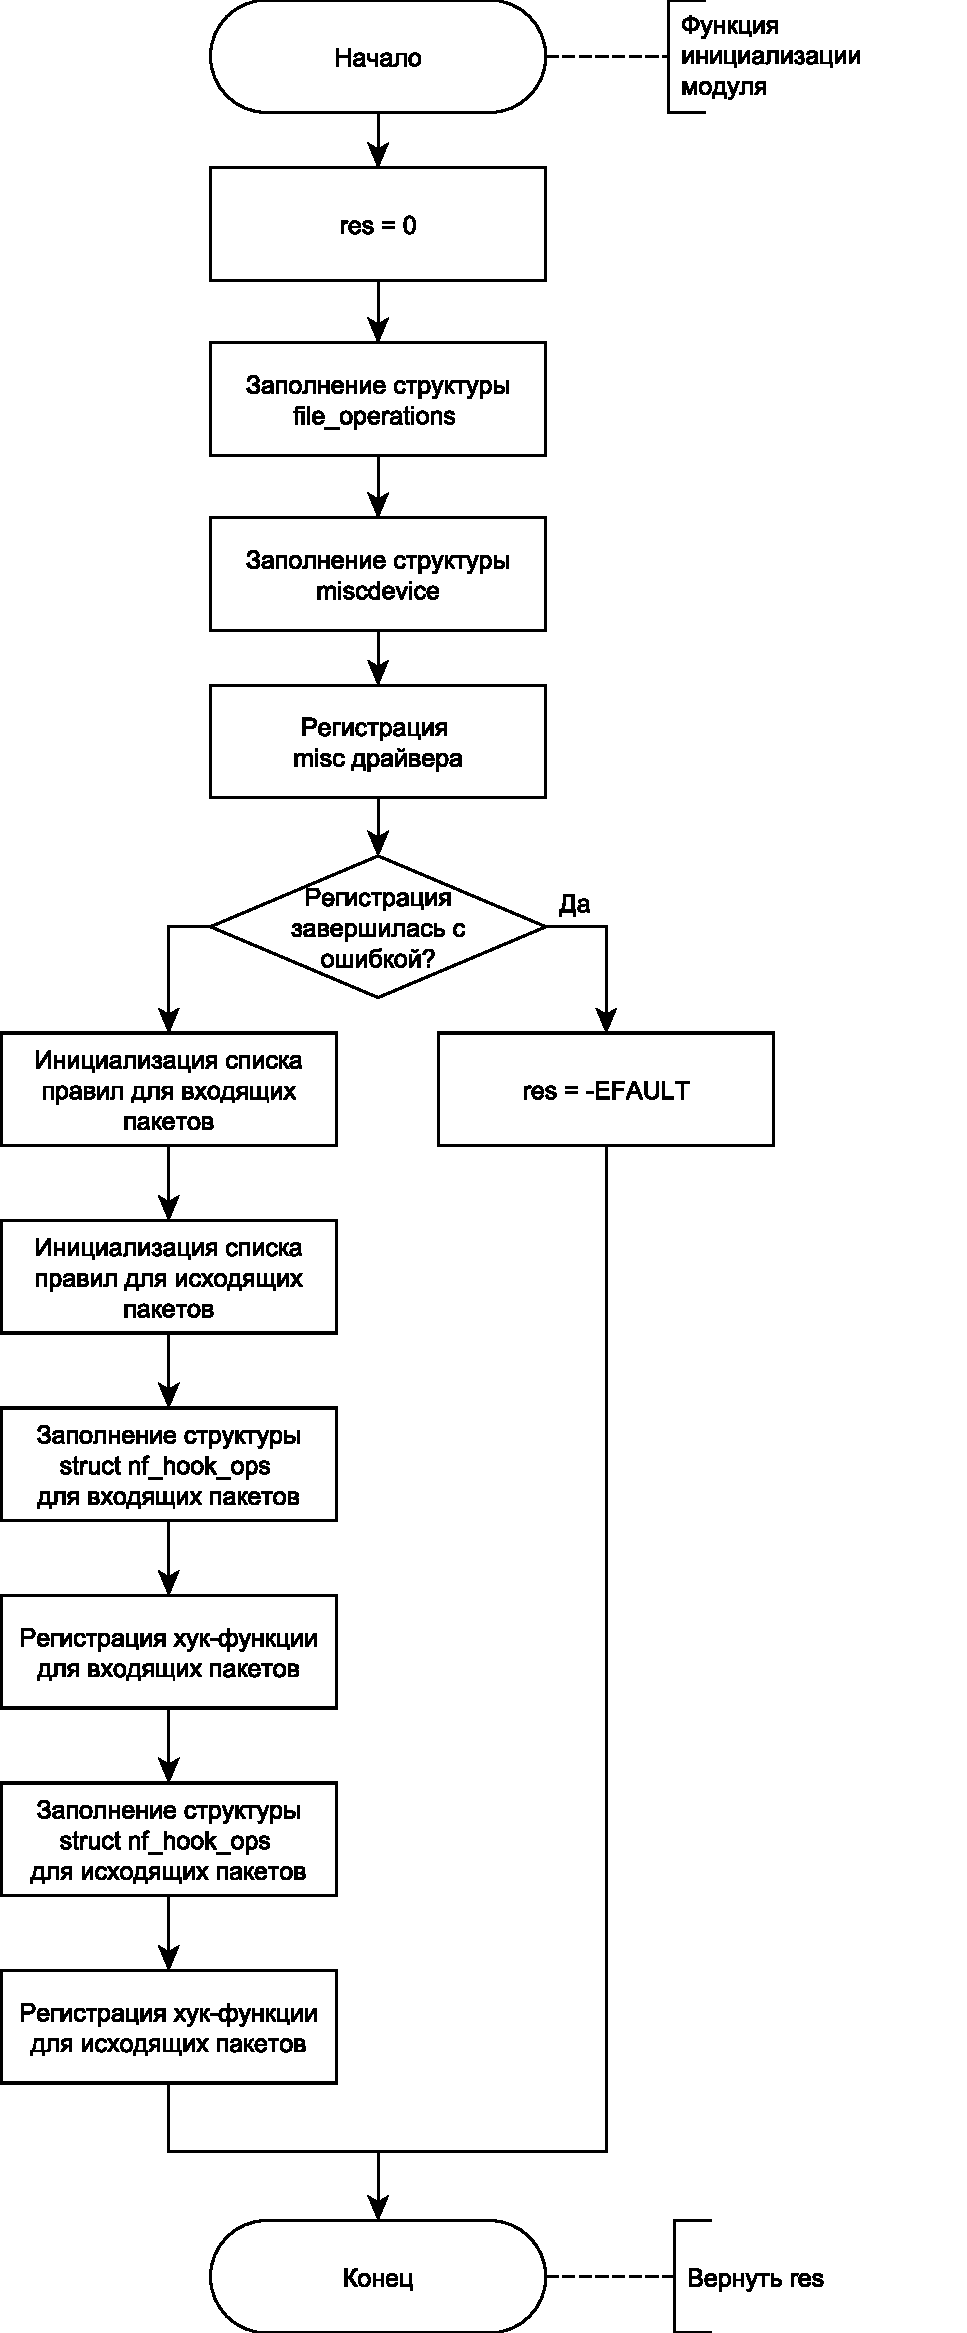
\includegraphics[scale = 0.6]{img/init.pdf}}
		\caption{Схема алгоритма инициализации межсетевого экрана}
		\label{fig3:image}
	\end{center}
\end{figure}

\newpage

\subsection{Завершение работы межсетевого экрана}
При выгрузке необходимо освободить все ресурсы, которые были зарезервированы. Детально алгоритм завершения работы межсетевого экрана изложен на Рисунке \ref{fig4:image}.
\begin{figure}[h!]
	\begin{center}
		{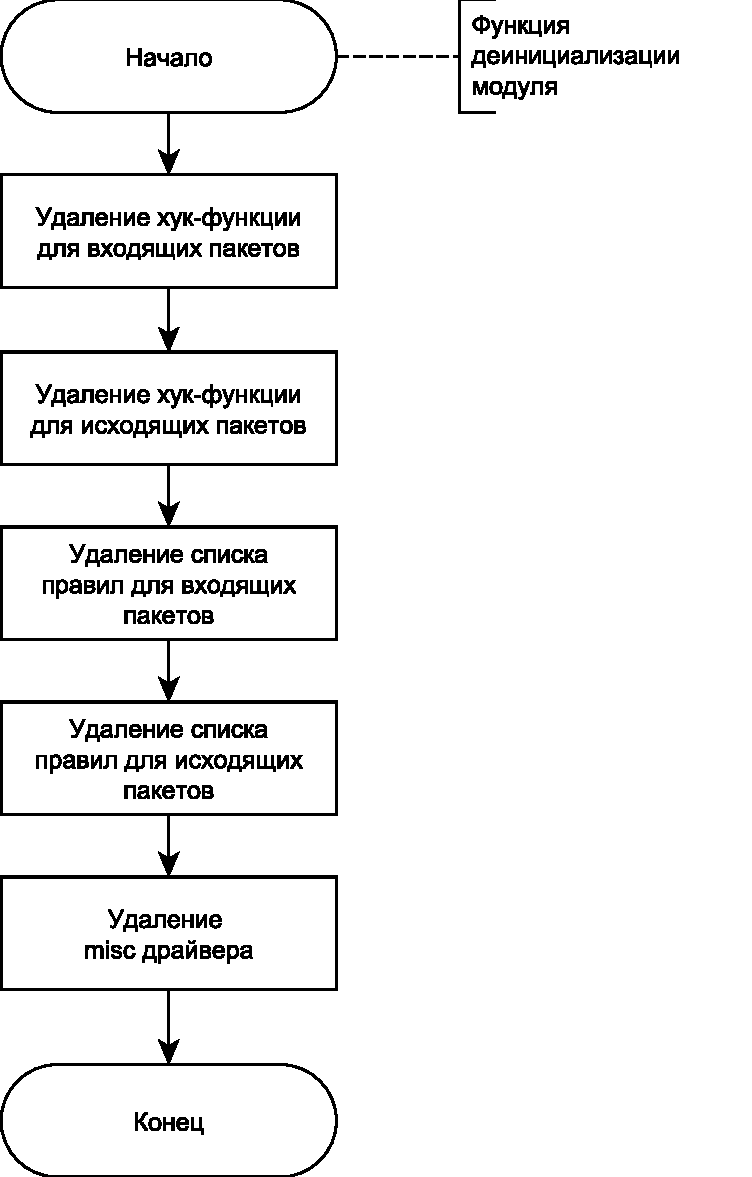
\includegraphics[scale = 0.6]{img/exit.pdf}}
		\caption{Схема алгоритма завершения работы межсетевого экрана}
		\label{fig4:image}
	\end{center}
\end{figure}

\subsection{Основные функции, определяемые в struct file\_operations}
При инициализации одним из первых действий -- заполнение структуры \textbf{struct file\_operations}, в которой определяются функции для работы с файлами. В рамках поставленной задачи необходимо указать свои функции read (для того, чтобы получить список всех правил), write (используется для обработки нового правила). 

На Рисунках \ref{fig5:image} -- \ref{fig6:image} приведены их схемы.
\begin{figure}[h!]
	\begin{center}
		{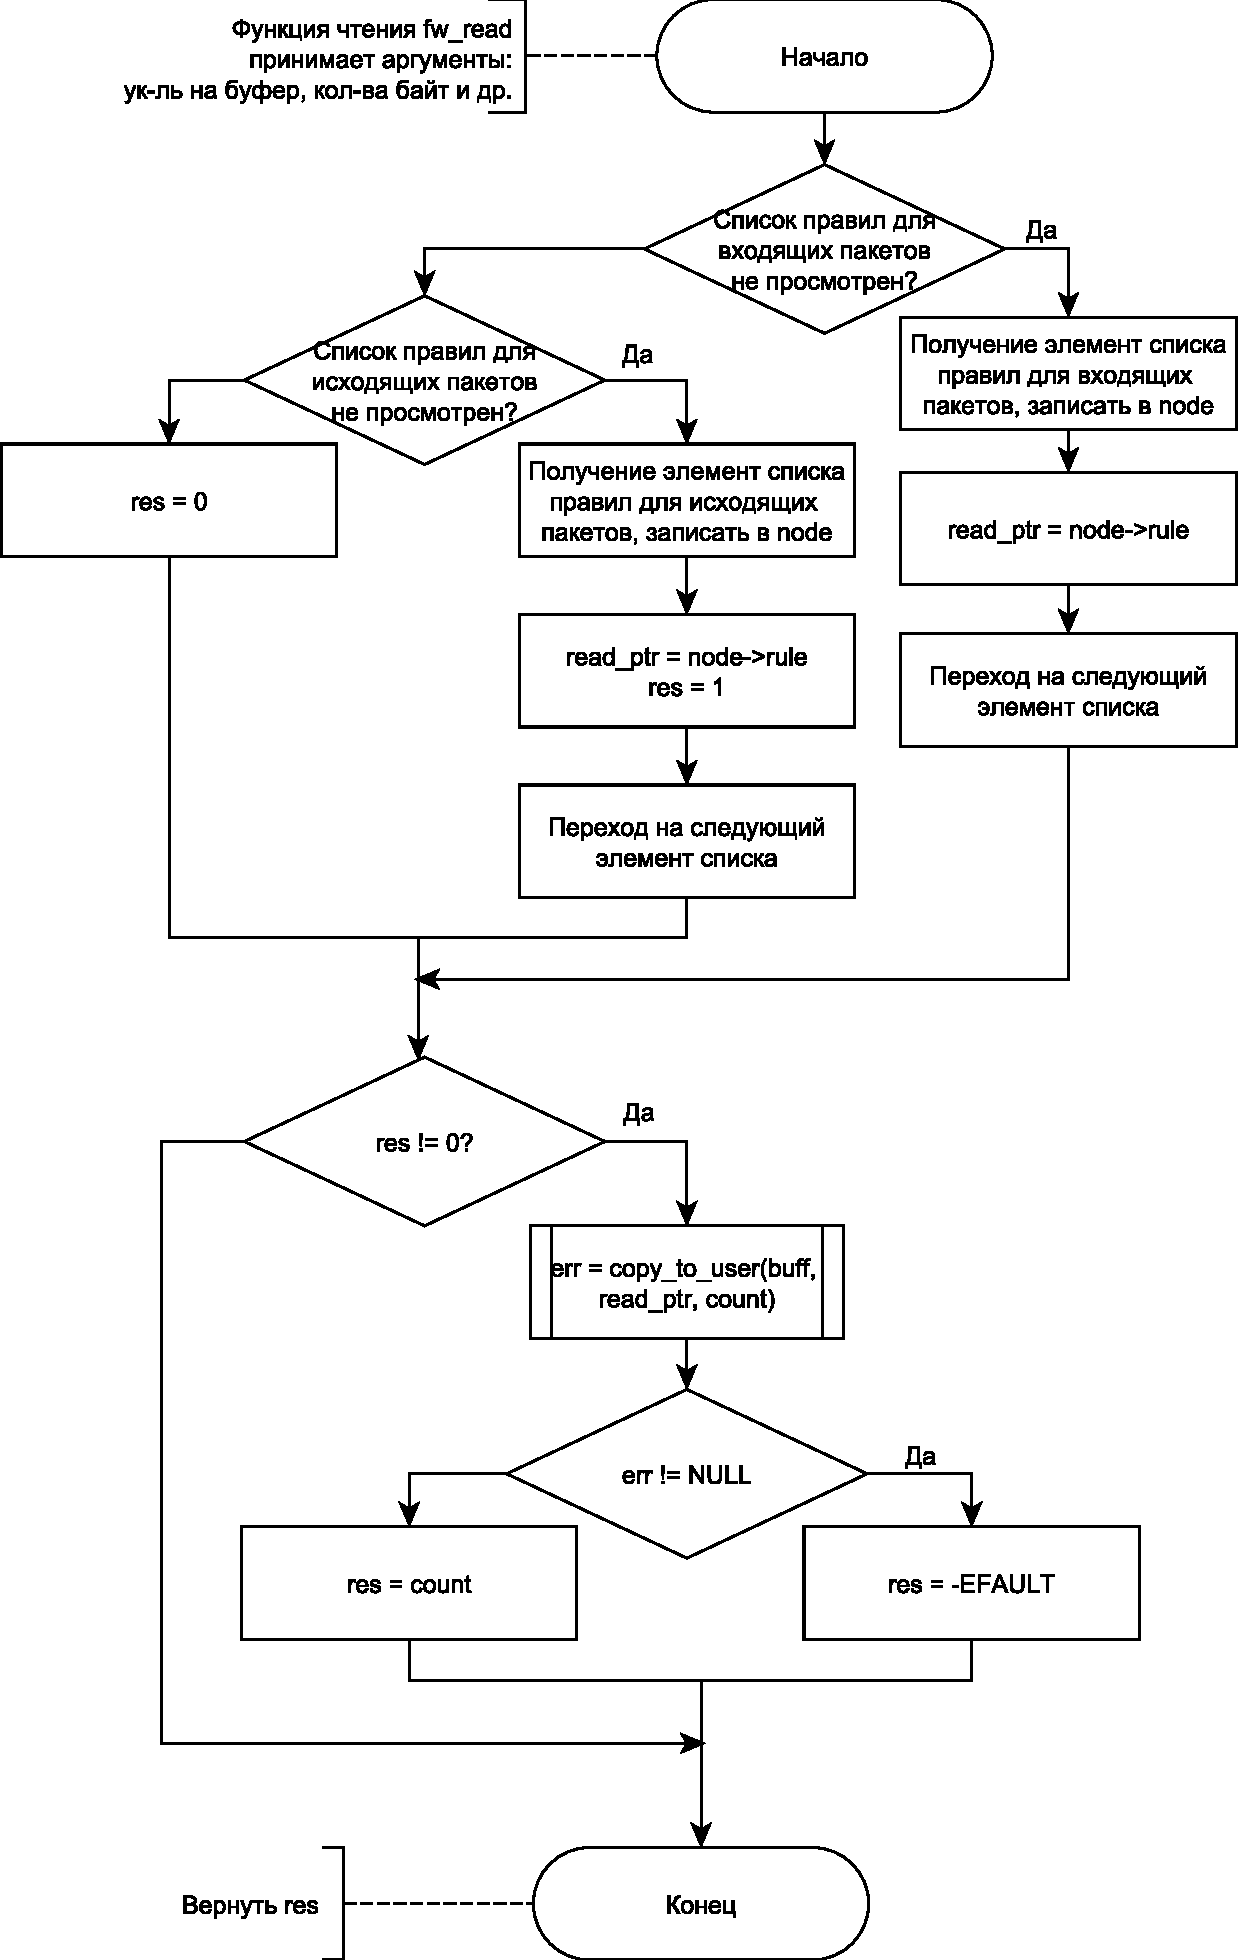
\includegraphics[scale = 0.63]{img/read.pdf}}
		\caption{Схема алгоритма чтения правил}
		\label{fig5:image}
	\end{center}
\end{figure}

\begin{figure}[h!]
	\begin{center}
		{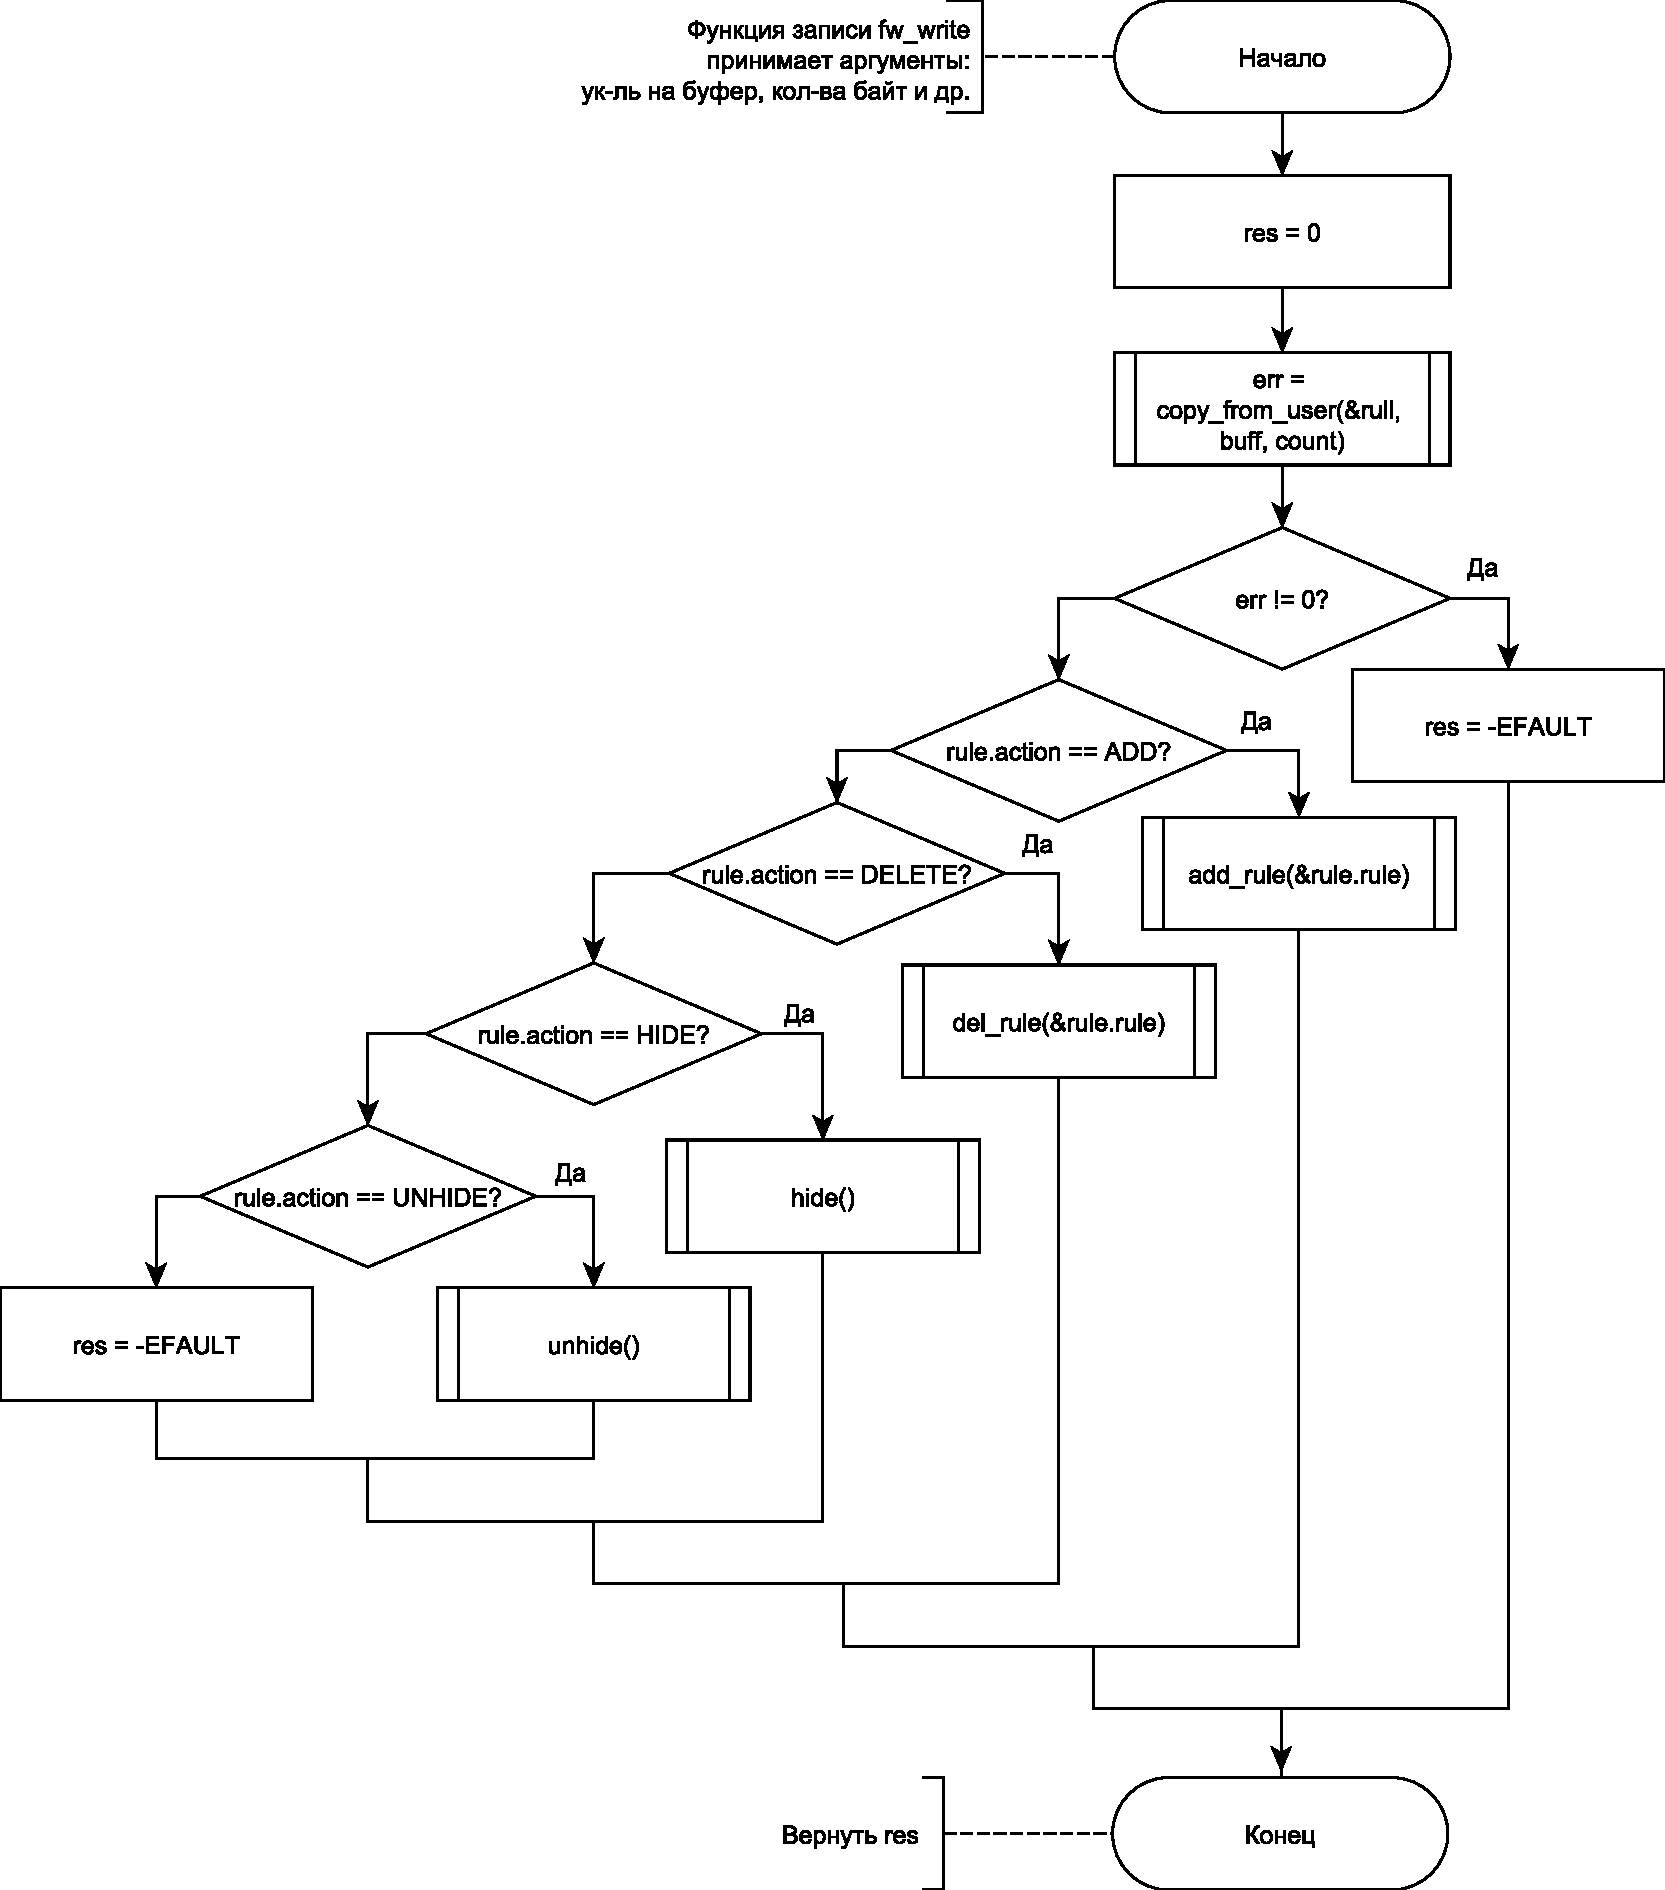
\includegraphics[scale = 0.6]{img/write.pdf}}
		\caption{Схема алгоритма записи правила}
		\label{fig6:image}
	\end{center}
\end{figure}

\newpage

\subsection{Функции добавления и удаления правил}
Пользователю предоставляется возможность добавить новое правило или удалить уже существующее. На Рисунках \ref{fig7:image} и \ref{fig8:image} показан общий подход к реализации каждой из возможностей.

\begin{figure}[h!]
	\begin{center}
		{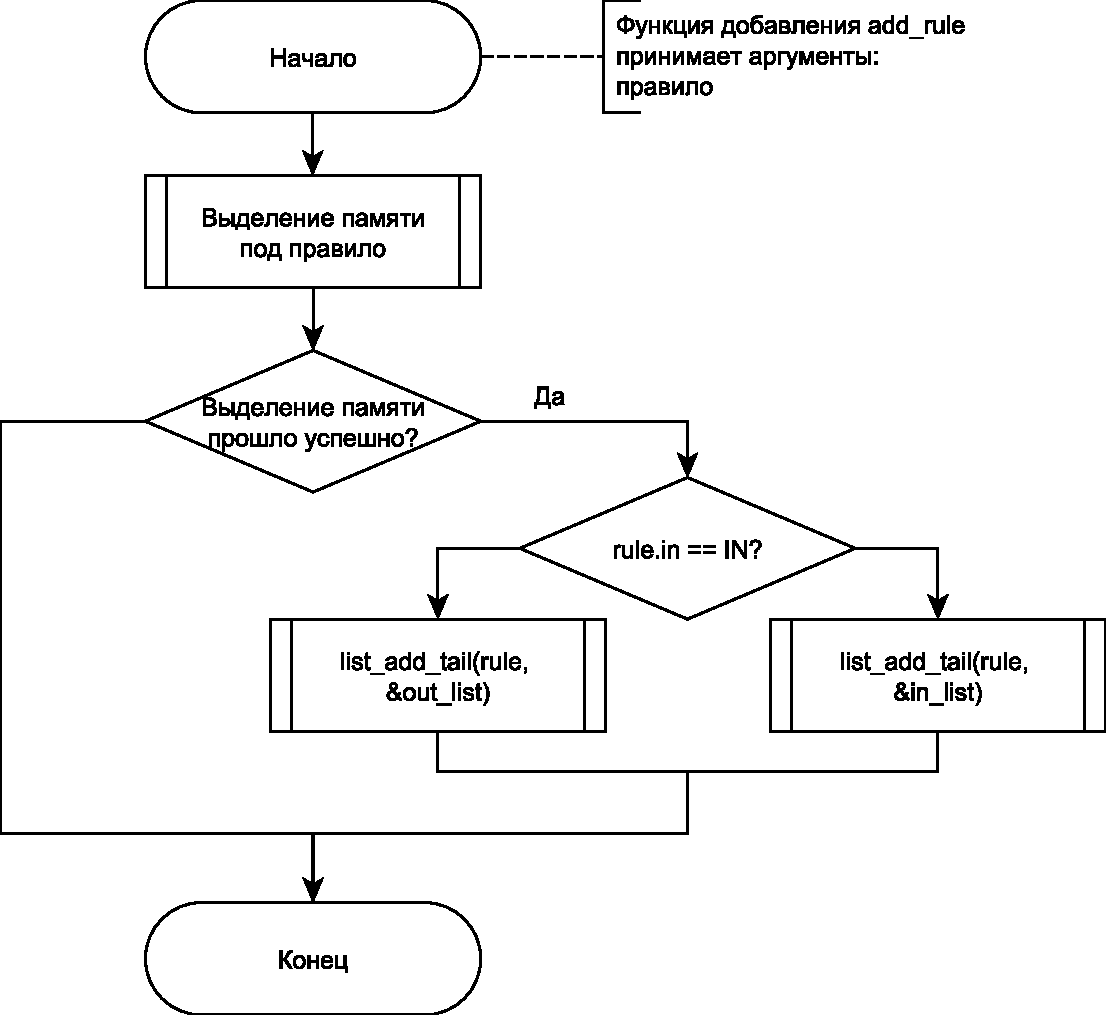
\includegraphics[scale = 0.6]{img/add_rule.pdf}}
		\caption{Схема алгоритма добавления нового правила}
		\label{fig7:image}
	\end{center}
\end{figure}

\begin{figure}[h!]
	\begin{center}
		{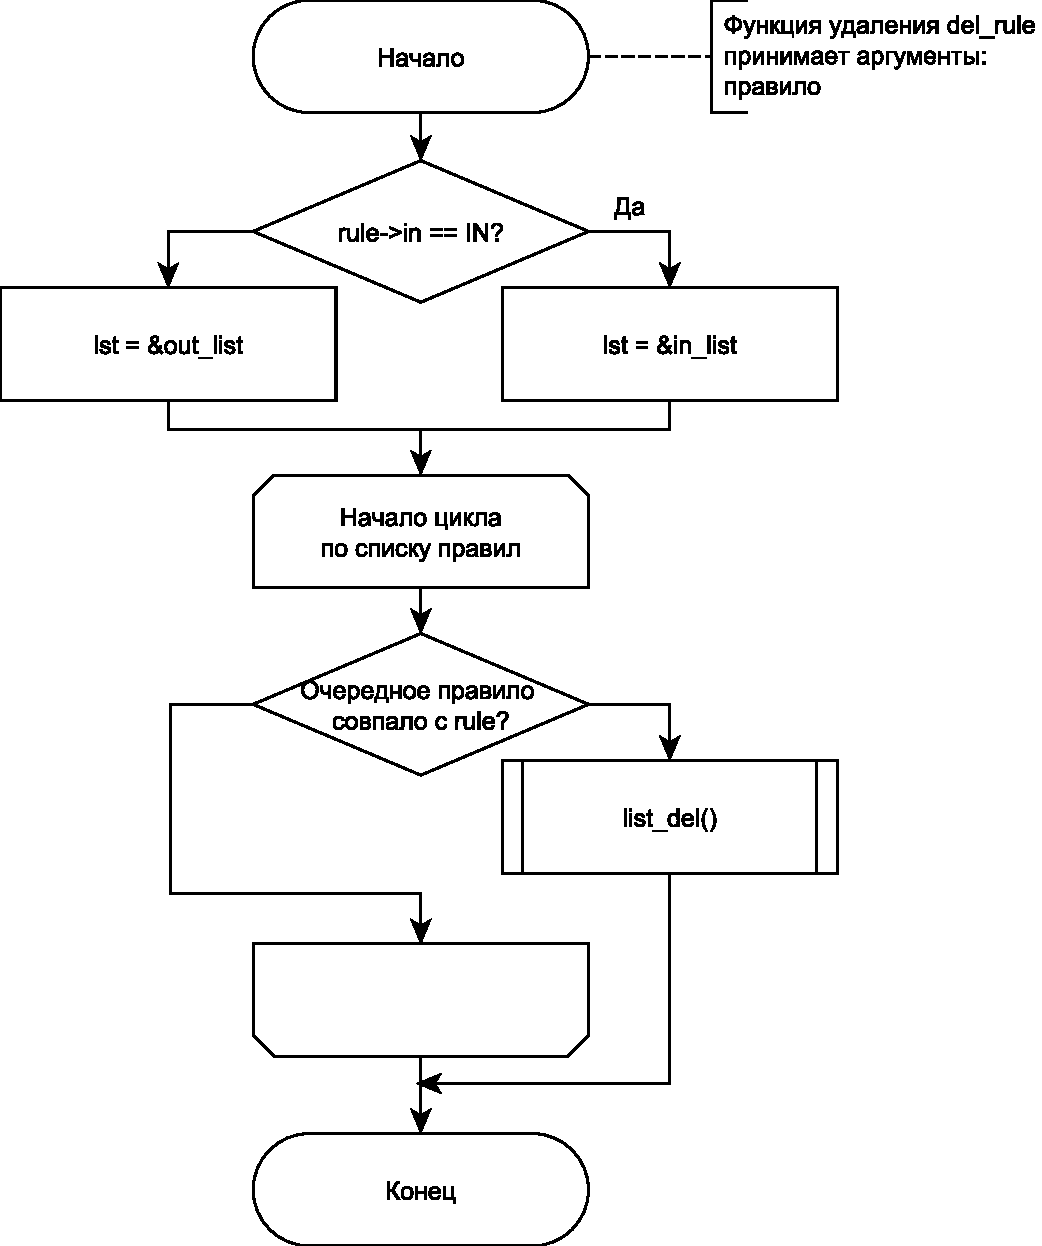
\includegraphics[scale = 0.55]{img/del_rule.pdf}}
		\caption{Схема алгоритма удаления правила}
		\label{fig8:image}
	\end{center}
\end{figure}

\pagebreak

\subsection{Функция фильтрации пакетов}
В процессе инициализации также происходит регистрация хук-функций, заданных в структуре \textbf{struct nf\_hook\_ops}. 

В рамках поставленной задачи регистрируются две функции: для обработки входящих и исходящих пакетов. Поскольку главное их отличие -- направление анализируемых единиц, то рекомендуется реализовать одну функцию, в которую подаётся соответствующий список правил. Детали представлены на Рисунках \ref{fig9:image} -- \ref{fig22:image}.

\begin{figure}[h!]
	\begin{center}
		{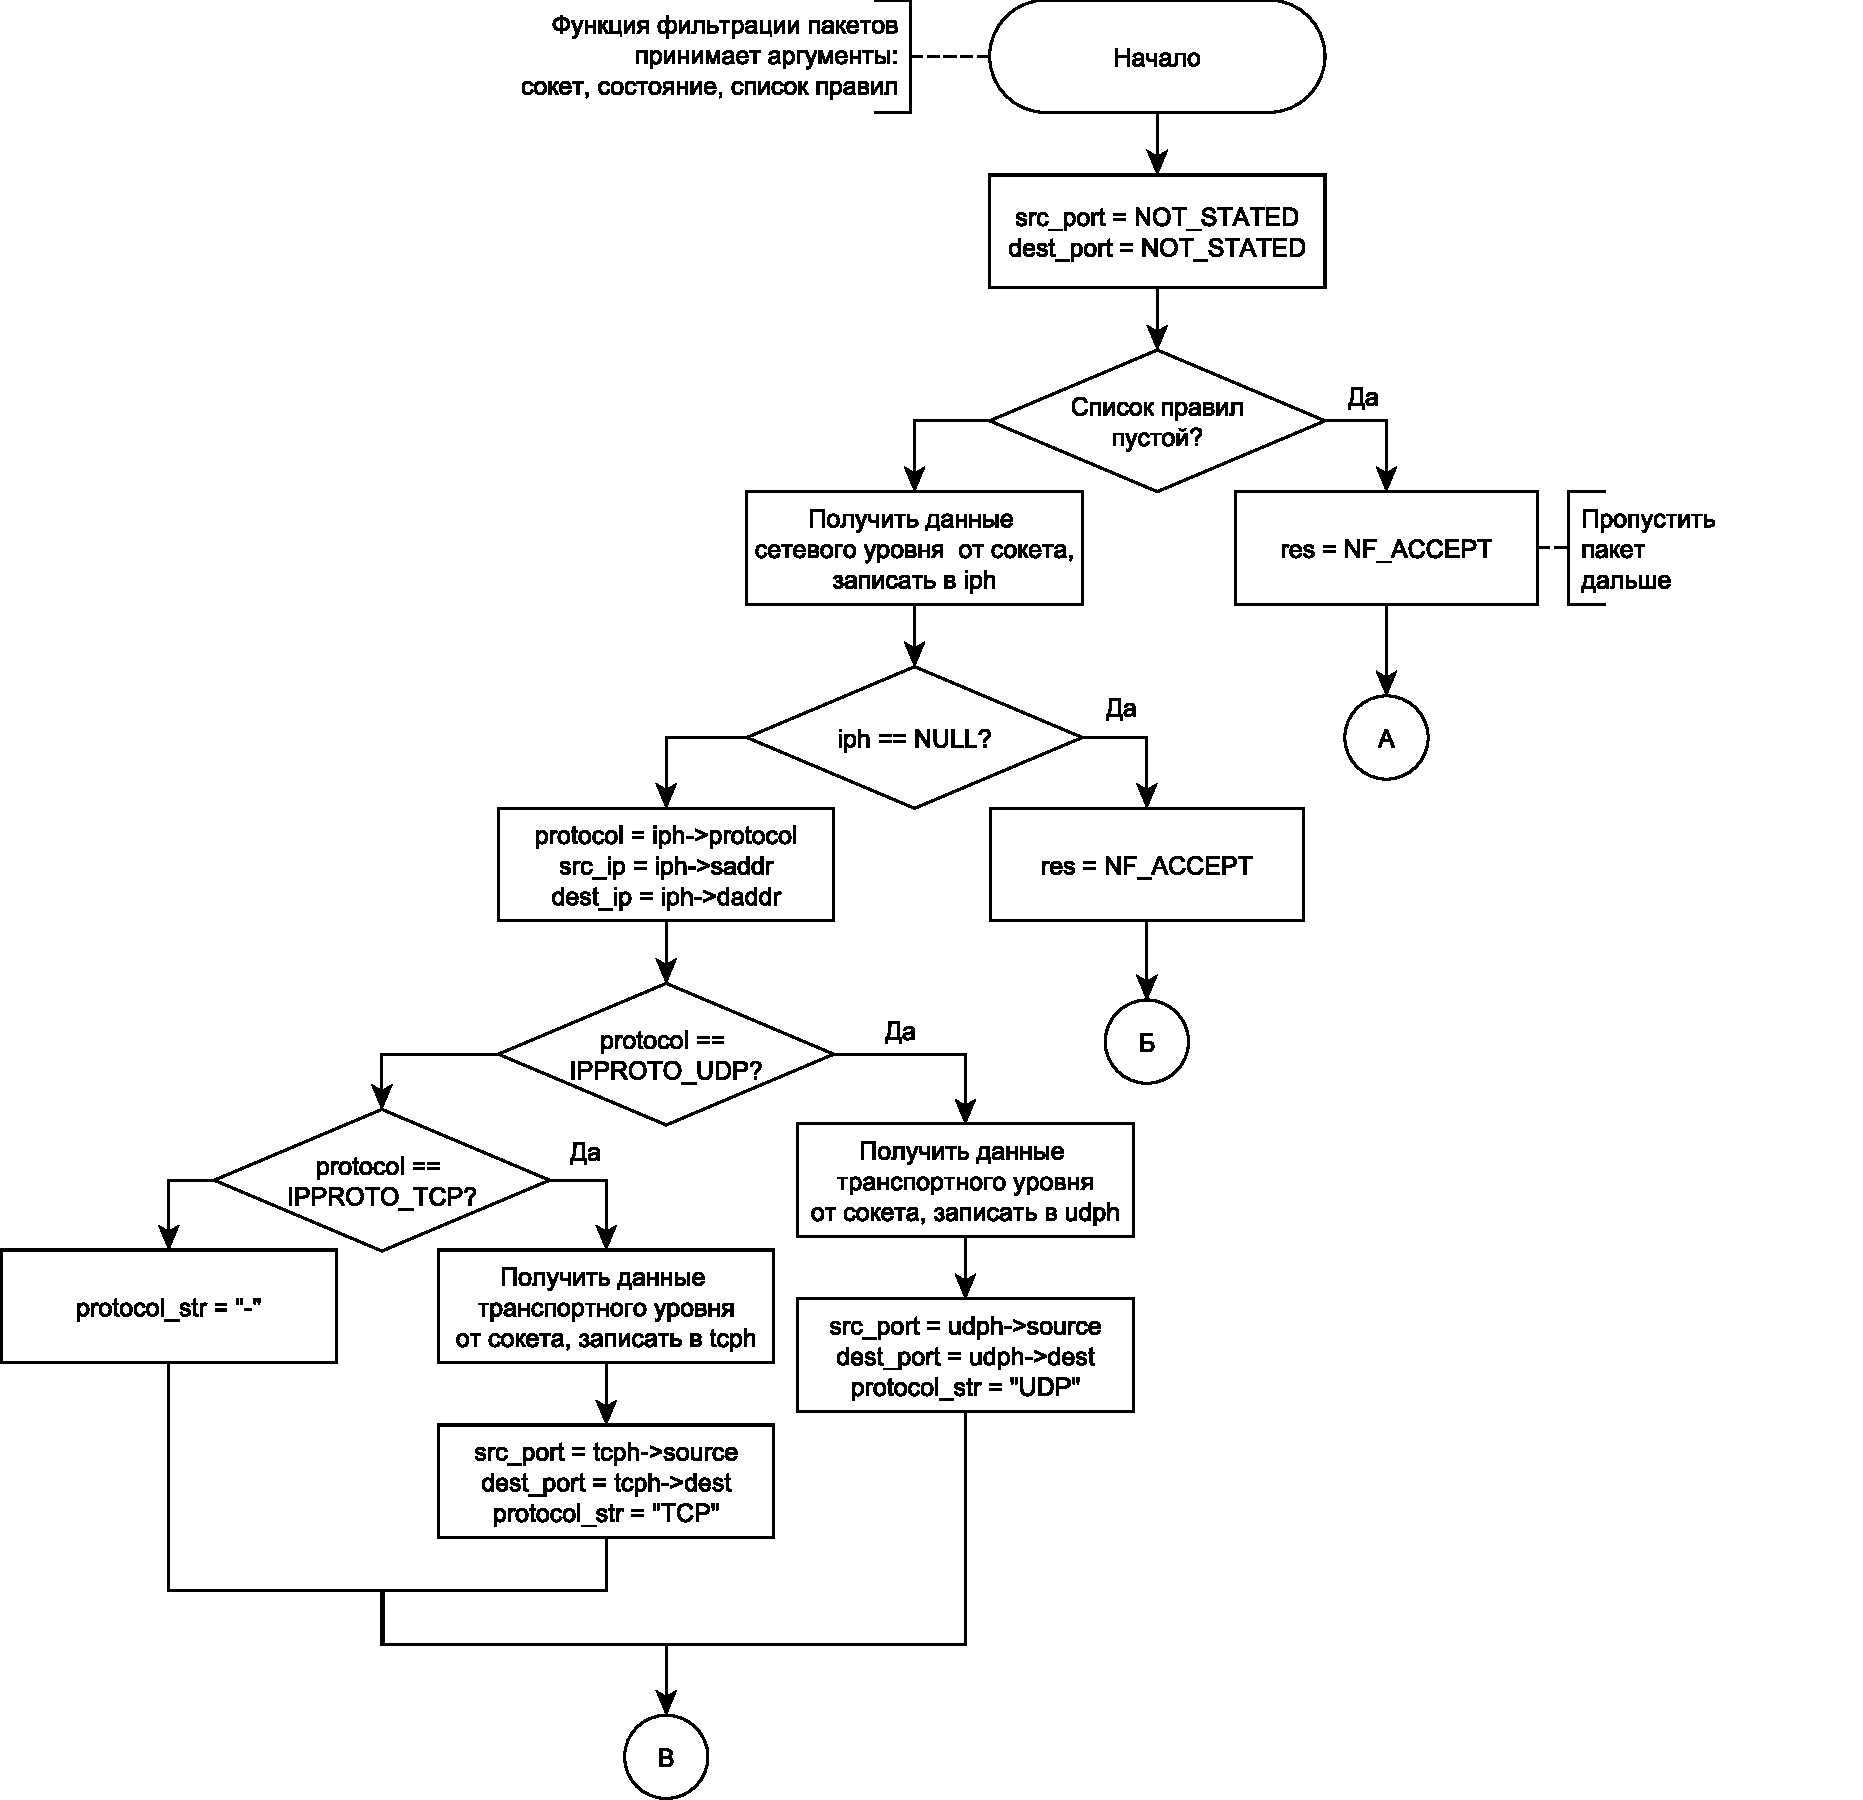
\includegraphics[scale = 0.55]{img/filter1.pdf}}
		\caption{Схема алгоритма фильтрации пакетов}
		\label{fig9:image}
	\end{center}
\end{figure}

\begin{figure}[h!]
	\begin{center}
		{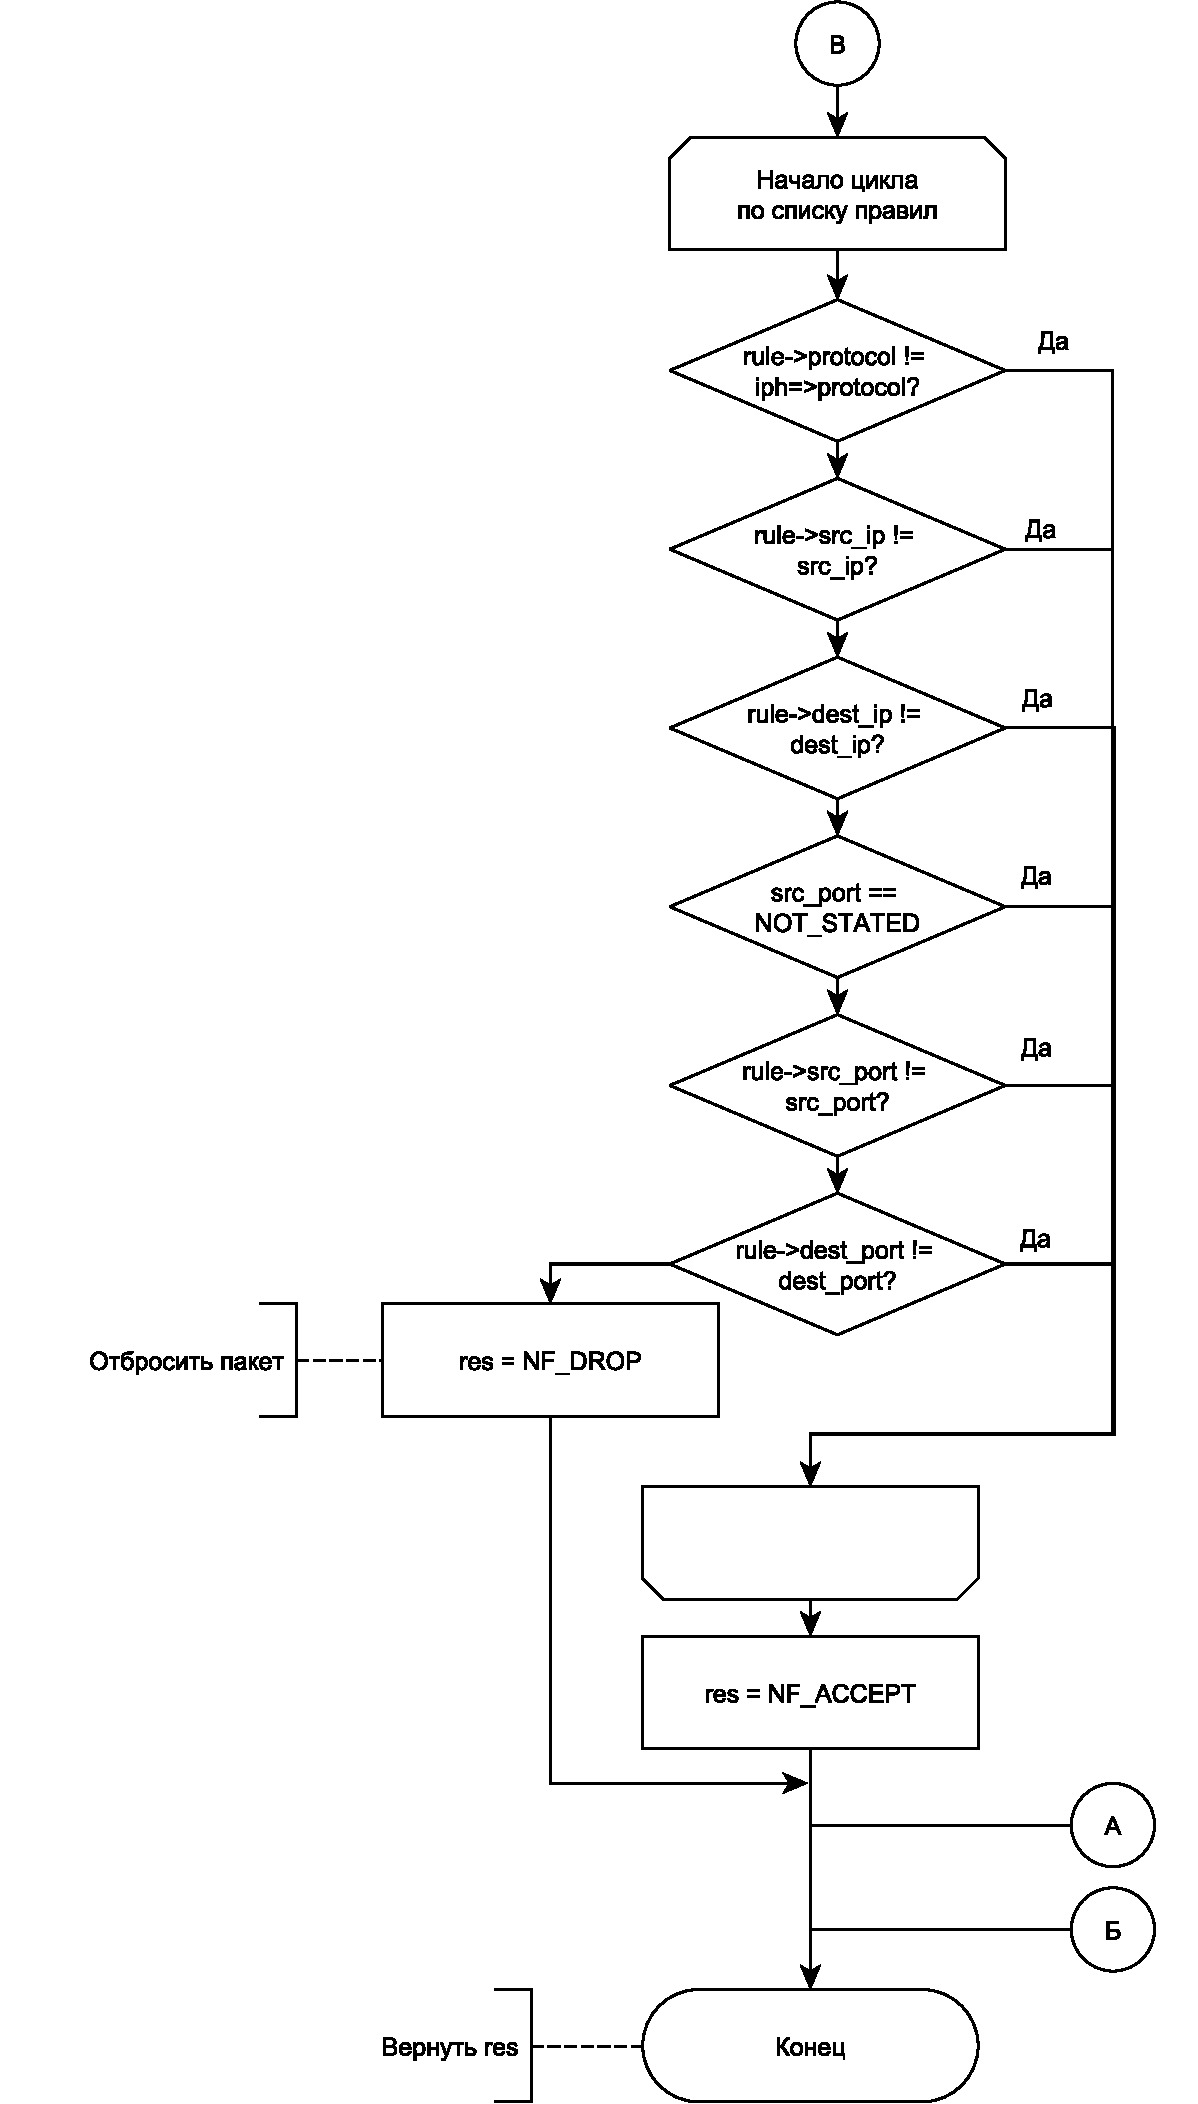
\includegraphics[scale = 0.55]{img/filter2.pdf}}
		\caption{Схема алгоритма фильтрации пакетов (продолжение 1)}
		\label{fig10:image}
	\end{center}
\end{figure}

\begin{figure}[h!]
	\begin{center}
		{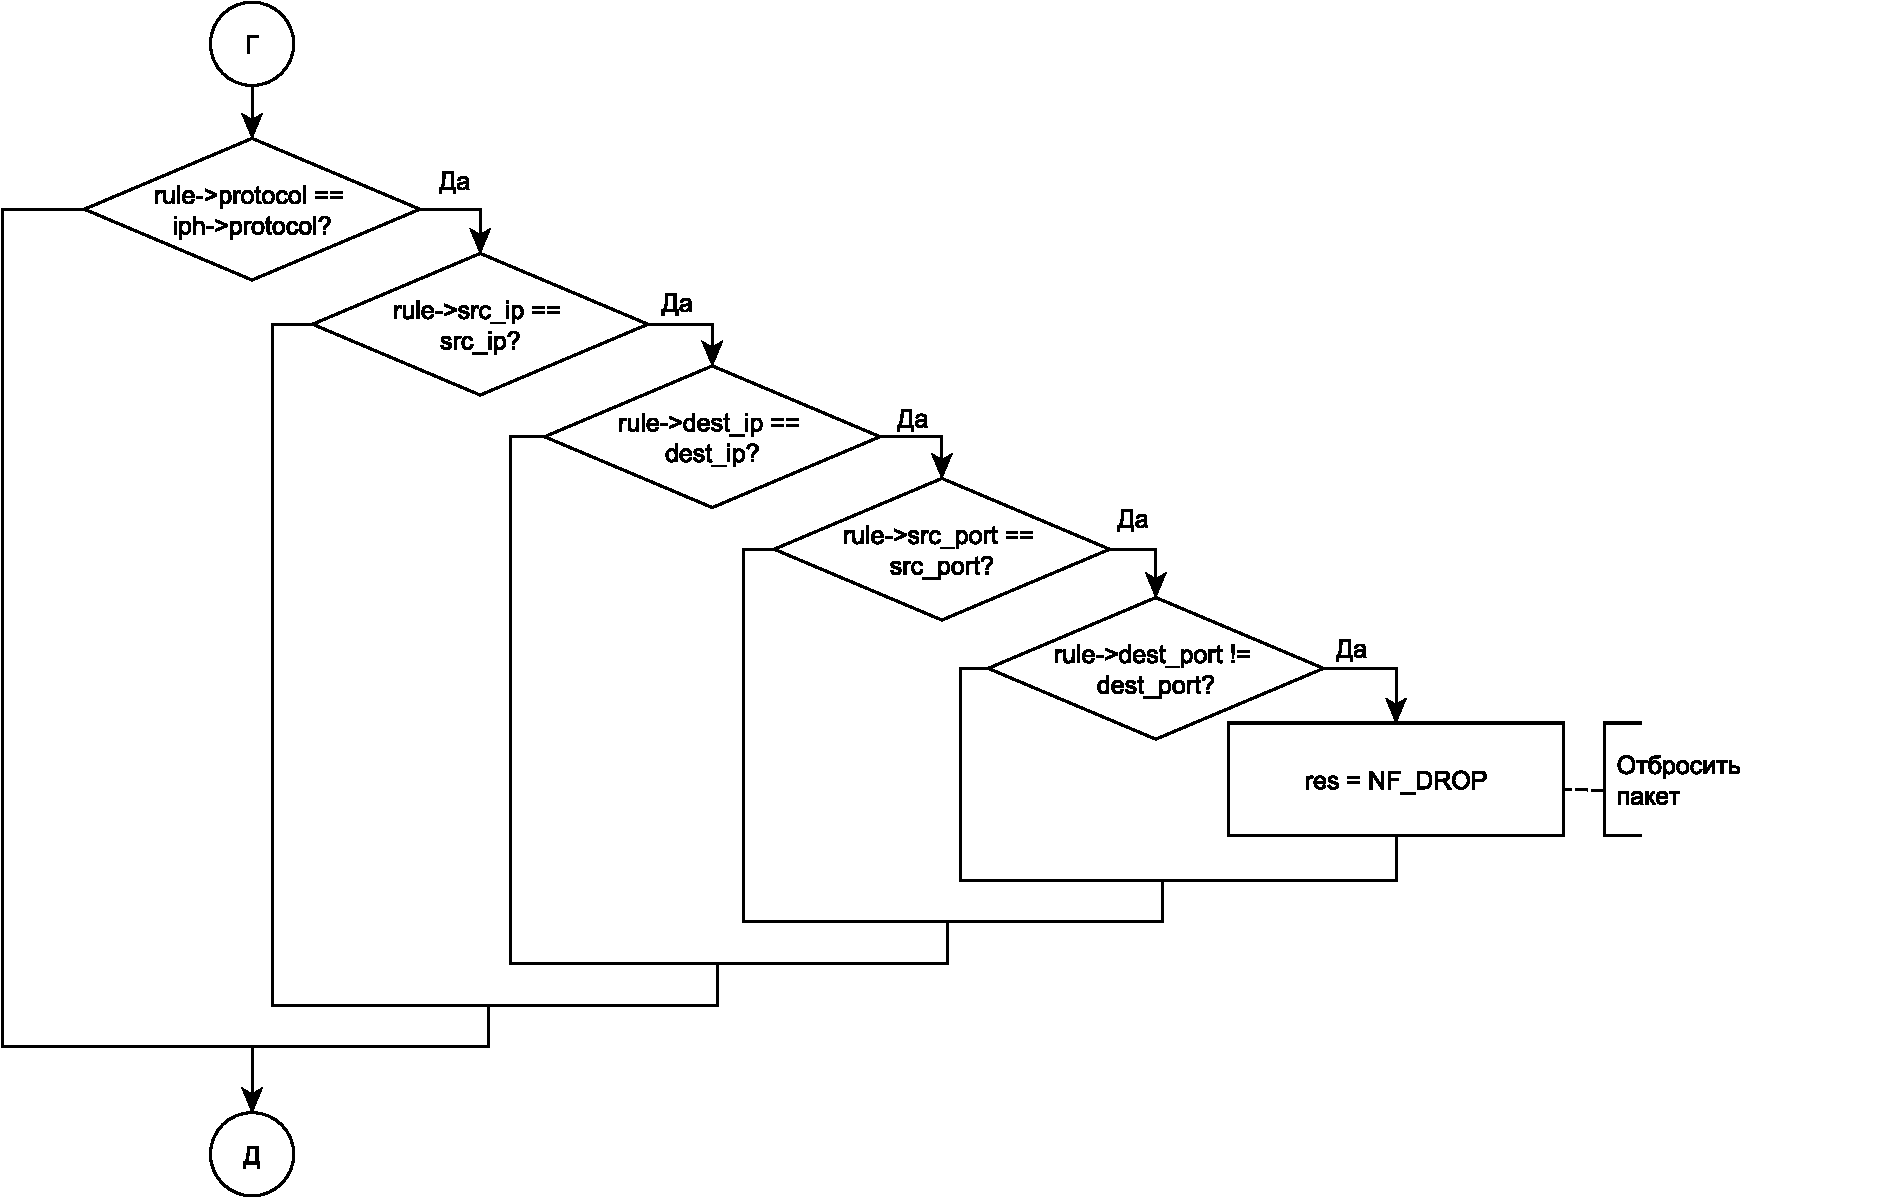
\includegraphics[scale = 0.55]{img/ifs.pdf}}
		\caption{Схема алгоритма фильтрации пакетов (продолжение 2)}
		\label{fig22:image}
	\end{center}
\end{figure}

\subsection{Выводы}
В разделе рассмотрены требования к программе, основные сведения о модуле, предоставлены схемы, описывающие ключевые моменты в его работе.
